%!TeX root=../tese.tex
%("dica" para o editor de texto: este arquivo é parte de um documento maior)
% para saber mais: https://tex.stackexchange.com/q/78101

\chapter{MSF totalmente dinâmica}
\label{chapter:fully-MSF}

Neste capítulo, consideraremos o problema da \textbf{MSF dinâmica}, onde queremos manter uma MSF em um grafo dinâmico. Estudaremos um algoritmo para MSF dinâmica. Como este algoritmo não foi implementado em nosso estudo, apresentaremos apenas a ideia por trás dele, de como podemos manter o peso mínimo de uma MSF de um grafo $G$ dando suporte à adição e remoção de arestas. Inicialmente, será descrito o funcionamento das \textbf{top trees}, estruturas de dados que serão usadas na manutenção da MSF dinâmica. Estas estruturas estão descritas na Seção~2.2 do artigo de Holm, de Lichtenberg e Thorup~\cite{jacob_holm}.

\section{Top trees}

Antes de definir uma top tree, precisamos definir alguns conceitos.
Seja um par ($T$, $\partial T$), onde $T$ é uma árvore e $\partial T$ é um conjunto que contém no máximo dois vértices de $T$, que são chamados \textbf{vértices da fronteira} (\textit{external boundary vertices}), como se pode ver na Figura~\ref{fig:top-tree-pair-representation}.

\begin{figure}[H]
    \centering
    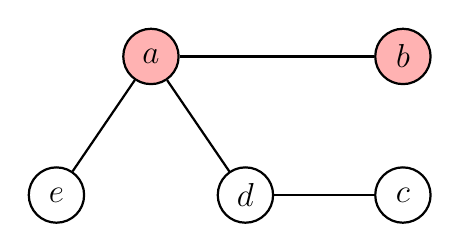
\begin{tikzpicture}
        [scale=0.8, node/.style={circle,draw,minimum size=2em, thick, font=\large},
        edge/.style={thick, black},
        reserve/.style={red, thick},
        removed/.style={black, thick, dashed}, 
        inner sep=0pt]

        \node[node, fill=red!30] (a) at (0,1.5) {$a$};
        \node[node, fill=red!30] (b) at (4,1.5) {$b$};
        \node[node] (c) at (4,-0.7) {$c$};
        \node[node] (d) at (1.5,-0.7) {$d$};
        \node[node] (e) at (-1.5,-0.7) {$e$};

        \draw[edge] (a) -- (b) node[midway, above] {};
        \draw[edge] (c) -- (d) node[midway, above] {};
        \draw[edge] (d) -- (a) node[midway, above] {};
        \draw[edge] (a) -- (e) node[midway, above] {};

    \end{tikzpicture}
    \caption{Uma árvore $T$ com um conjunto $\partial T$ destacado em vermelho}
    \label{fig:top-tree-pair-representation}
\end{figure}

Para qualquer subárvore $C$ de $T$, seja um conjunto $\partial_{(T, \partial T)}C$, que são vértices de $C$ que estão ou em $\partial T$ ou são incidentes a uma aresta de $T$ saindo de $C$. Chamamos o conjunto $\partial_{T, \partial T}C$ de vértices da fronteira de $C$. Veja o exemplo da Figura~\ref{fig:top-tree-subtree-option1}.

\begin{figure}[H]
    \centering
    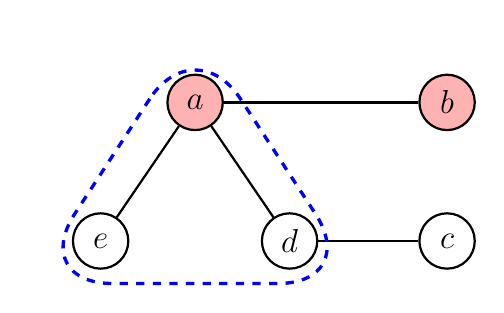
\begin{tikzpicture}
        [scale=0.8, node/.style={circle,draw,minimum size=2em, thick, font=\large},
        edge/.style={thick, black},
        reserve/.style={red, thick},
        removed/.style={black, thick, dashed}, 
        inner sep=0pt]

        \node[node, fill=red!30] (a) at (0,1.5) {$a$};
        \node[node, fill=red!30] (b) at (4,1.5) {$b$};
        \node[node] (c) at (4,-0.7) {$c$};
        \node[node] (d) at (1.5,-0.7) {$d$};
        \node[node] (e) at (-1.5,-0.7) {$e$};

        \draw[edge] (a) -- (b) node[midway, above] {};
        \draw[edge] (c) -- (d) node[midway, above] {};
        \draw[edge] (d) -- (a) node[midway, above] {};
        \draw[edge] (a) -- (e) node[midway, above] {};
        
        % P1: Top Vertex (above node 'a')
        \coordinate (P1) at ([yshift=20pt]a.north); 
        
        % P2: Bottom-Left Vertex (left of 'e' and slightly below it, using calc for precision)
        \coordinate (P2) at ([xshift=-23pt, yshift=-10pt]e.south west);
        
        % P3: Bottom-Right Vertex (right of 'd' and slightly below it, using calc for precision)
        \coordinate (P3) at ([xshift=23pt, yshift=-10pt]d.south east);

        % --- Draw the Dashed Triangular Outline ---
        
        % Connect the invisible coordinates with rounded corners
        \draw[dashed, very thick, blue, rounded corners=30pt] 
            (P1) -- (P2) -- (P3) -- cycle;

        % \draw[dashed, thick, red] (e) -- (a) -- (d) -- cycle;
    \end{tikzpicture}
    \caption{Uma árvore $T$ com um conjunto $\partial T$ marcado em vermelho. A região demarcada em azul representa uma subárvore $C$ contendo os vértices $a$, $e$ e $d$ e as arestas $ae$ e $ad$. Neste exemplo, note que os vértices da fronteira de $C$ são $a$ e $d$.}
    \label{fig:top-tree-subtree-option1}
\end{figure}

Uma subárvore $C$ é chamada de \textbf{cluster} de ($T$, $\partial T$) se o número de vértices da fronteira de $C$ é no máximo dois. Assim, por definição, $T$ é um cluster dele mesmo, com $\partial_{(T, \partial T)}T = \partial T$. Além disso, qualquer aresta de $T$ é um cluster de ($T$, $\partial T$). A subárvore $C$ da Figura~\ref{fig:top-tree-subtree-option1} acima é um cluster, pois ela possui apenas dois vértices da fronteira.

Além disso, se $R$ é uma subárvore de $C$, então $R$ é um cluster  
 de ($C$, $\partial_{(T, \partial T)} C$) se, e somente se, $R$ é um cluster de $(T, \partial T)$. Podemos ver essa situação no exemplo da Figura~\ref{fig:top-tree-cluster-of-cluster}. Para simplificar, denotaremos $\partial_{(T, \partial T)}$ como $\partial$ a partir de agora.

 \begin{figure}[H]
    \centering
    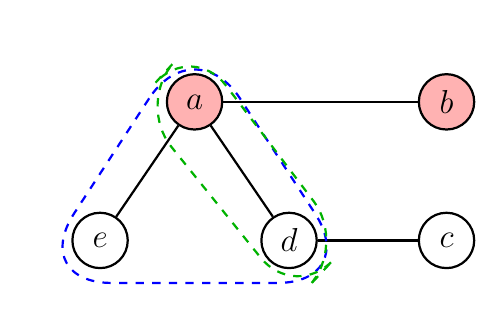
\begin{tikzpicture}
        [scale=0.8, node/.style={circle,draw,minimum size=2em, thick, font=\large},
        edge/.style={thick, black},
        reserve/.style={red, thick},
        removed/.style={black, thick, dashed}, 
        inner sep=0pt]

        \node[node, fill=red!30] (a) at (0,1.5) {$a$};
        \node[node, fill=red!30] (b) at (4,1.5) {$b$};
        \node[node] (c) at (4,-0.7) {$c$};
        \node[node] (d) at (1.5,-0.7) {$d$};
        \node[node] (e) at (-1.5,-0.7) {$e$};

        \draw[edge] (a) -- (b) node[midway, above] {};
        \draw[edge] (c) -- (d) node[midway, above] {};
        \draw[edge] (d) -- (a) node[midway, above] {};
        \draw[edge] (a) -- (e) node[midway, above] {};
        
        % P1: Top Vertex (above node 'a')
        \coordinate (P1) at ([yshift=20pt]a.north); 
        
        % P2: Bottom-Left Vertex (left of 'e' and slightly below it, using calc for precision)
        \coordinate (P2) at ([xshift=-23pt, yshift=-10pt]e.south west);
        
        % P3: Bottom-Right Vertex (right of 'd' and slightly below it, using calc for precision)
        \coordinate (P3) at ([xshift=23pt, yshift=-10pt]d.south east);


        \draw[dashed, thick, blue, rounded corners=30pt] 
            (P1) -- (P2) -- (P3) -- cycle;
        % G1: Top-Left point (relative to 'a')
  
        % Top-Left corner (above and to the left of 'a')
        \coordinate (DR1) at ([xshift=-10pt, yshift=18pt]a.north east); 
        
        % Bottom-Left corner (below and to the left of 'a', near 'e')
        \coordinate (DR2) at ([xshift=-17pt, yshift=-10pt]a.north west); 
        
        % Bottom-Right corner (below and to the right of 'd', near 'c')
        \coordinate (DR3) at ([xshift=12pt, yshift=-18pt]d.south west); 
        
        % Top-Right corner (above and to the right of 'd')
        \coordinate (DR4) at ([xshift=17pt, yshift=7pt]d.south east); 

        % --- Draw the Dashed Green Diagonal Rectangle ---
        \draw[dashed, thick, green!70!black, rounded corners=20pt] 
            (DR1) -- (DR2) -- (DR3) -- (DR4) -- cycle;

        % \draw[dashed, thick, red] (e) -- (a) -- (d) -- cycle;
    \end{tikzpicture}
    \caption{A região demarcada em azul representa a subárvore $C$ de $T$, e é cluster de $(T, \partial T)$. Já a região demarcada em verde representa uma subárvore $R$ de $C$, e é cluster de $(C, \partial C)$ e de $(T, \partial T)$.}
    \label{fig:top-tree-cluster-of-cluster}
\end{figure}

Dizemos que clusters $A$ e $B$ são vizinhos se eles compartilham um único vértice e se $A \cup B$ é um cluster. Finalmente, definimos uma \textbf{top tree} $\mathcal{T}$ do par ($T$, $\partial T$) como sendo uma árvore binária que respeita o seguinte:

\begin{itemize}
    \item Os vértices de $\mathcal{T}$ são os clusters de ($T$, $\partial T$);
    \item As folhas de $\mathcal{T}$ são as arestas de $T$;
    \item Se $C$ é pai de $A$ e de $B$ em $\mathcal{T}$, então $C = A \cup B$ e $A$ e $B$ são vizinhos;
    \item A raiz de $\mathcal{T}$ é a própria árvore $T$.
\end{itemize}

Para um cluster $C$, os vértices em $C\backslash \partial C$ são chamados de \textbf{vértices internos}. Se $a$ e $b$ são vértices da fronteira de $C$, o caminho entre $a$ e $b$ em $C$ se chama \textbf{caminho de cluster} e o denotamos por $\pi(C)$. Se $a \neq b$, o cluster é chamado de \textbf{cluster-caminho}. 

Dizemos que o cluster $C$ é \textbf{ancestral de caminho} do cluster $D$ e $D$ é chamado de \textbf{descendente de caminho} de $C$ se ambos forem cluster-caminhos e $\pi(D) \subseteq \pi(C)$. Note que cada aresta $e \in \pi(C)$ é um descendente de caminho de $C$. Um filho que é descendente de caminho é um \textbf{filho de caminho}. Na Figura~\ref{fig:clusters-formation-cases}, apresentamos os quatro casos quando fazemos a união de dois clusters. Em (1), temos dois filhos de caminho; em (2), temos um filho de caminho; e em (3) e (4), temos nenhum filho de caminho.


\begin{figure}[H]
    \centering
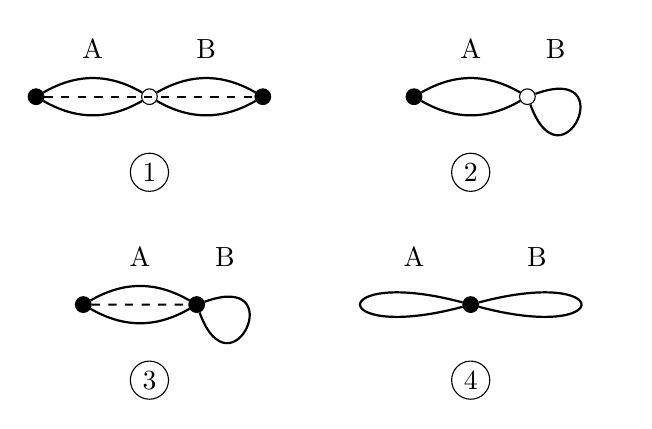
\begin{tikzpicture}[scale=1.2,
    every node/.style={circle, draw, inner sep=2pt},
    boundary/.style={fill=black},
    internal/.style={fill=white},
    edge/.style={thick},
    dashededge/.style={thick, dashed}
]

% (1)
\node[draw=none] (A1) at (0.6,0.5) {A};
\node[draw=none] (B1) at (1.8,0.5) {B};

\node[boundary] (a1) at (0,0) {};
\node[internal] (b1) at (1.2,0) {};
\node[boundary] (c1) at (2.4,0) {};

\draw[edge, bend left=30] (a1) to (b1);
\draw[edge, bend right=30] (a1) to (b1);
\draw[edge, bend left=30] (b1) to (c1);
\draw[edge, bend right=30] (b1) to (c1);
\draw[dashededge] (a1) -- (c1);
\node at (1.2, -0.8) {1};

% (2)
\node[draw=none] (A2) at (4.6,0.5) {A};
\node[draw=none] (B2) at (5.5,0.5) {B};

\node[boundary] (a2) at (4,0) {};
\node[internal] (b2) at (5.2,0) {};

\draw[edge, bend left=30] (a2) to (b2);
\draw[edge, bend right=30] (a2) to (b2);
\draw[edge, in=290, out=20, looseness=20] (b2) to (b2);
%\draw[dashededge] (a2) -- (b2);
\node at (4.6, -0.8) {2};

% (3)
\node[draw=none] (A3) at (4,-1.7) {A};
\node[draw=none] (B3) at (5.3,-1.7) {B};

\node[boundary] (a3) at (0.5,-2.2) {};
\node[boundary] (b3) at (1.7,-2.2) {};

\draw[edge, bend left=30] (a3) to (b3);
\draw[edge, bend right=30] (a3) to (b3);
\draw[edge, in=290, out=20, looseness=20] (b3) to (b3);
\draw[dashededge] (a3) -- (b3);
\node at (1.2, -3) {3};

% (4)
\node[draw=none] (A4) at (1.1,-1.7) {A};
\node[draw=none] (B4) at (2,-1.7) {B};

\node[boundary] (a4) at (4.6, -2.2) {};
\draw[edge] (a4) edge[loop left, min distance=15mm, looseness=4] (a4);
\draw[edge] (a4) edge[loop right, min distance=15mm, looseness=4] (a4);
\node at (4.6, -3) {4};

\end{tikzpicture}
\caption{Representação da união de dois clusters $A$ e $B$ formando um cluster $C$, e seus quatro diferentes casos. Os vértices pretos são vértices da fronteira de $C$ após a união de $A$ e $B$. Já os vértices brancos são vértices da fronteira de $A$ e de $B$, que não são vértices da fronteira de $C$. A linha tracejada é o cluster-caminho formado entre os vértices da fronteira de $C$.}
    \label{fig:clusters-formation-cases}
\end{figure}

Ademais, se $a$ é um vértice de fronteira de $C$ e $C$ possui dois filhos $A$ e $B$, então $A$ é considerado o mais próximo de $a$ se $a \notin B$. Caso $\partial C = \partial A = \partial C$, então o cluster mais próximo é escolhido arbitrariamente. Dadas essas definições, podemos ilustrar como ficaria uma \textit{top tree} para a árvore $T$ da Figura~\ref{fig:tree-t}.

\begin{figure}[H]
    \centering
    \begin{tikzpicture}
        [scale=0.8, node/.style={circle,draw,minimum size=2em, thick, font=\large},
        edge/.style={thick, black},
        reserve/.style={red, thick},
        removed/.style={black, thick, dashed}, 
        inner sep=0pt]

        \node[node, fill=red!30] (five) at (0, 0) {$5$};
        \node[node, fill=red!30] (four) at (-4, -1) {$4$};
        \node[node] (seven) at (4, -1) {$7$};
        \node[node] (six) at (0, -2) {$6$};
        \node[node] (three) at (-5, -3.5) {$3$};
        \node[node] (one) at (-6, -6) {$1$};
        \node[node] (two) at (-4, -6) {$2$};
       
        \node[node] (eight) at (2, -3.5) {$8$};
        \node[node] (nine) at (6, -3.5) {$9$};
        \node[node] (ten) at (6, -6) {$10$};


        % tree edges (normal black edges)
        \draw[edge] (one) -- (three) node[midway, below, weight, yshift=2pt] {$a$};
        \draw[edge] (three) -- (two) node[midway, below, weight, yshift=2pt] {$b$};
        \draw[edge] (three) -- (four) node[midway, below, weight, yshift=2pt] {$c$};

        \draw[edge] (four) -- (five) node[midway, below, weight, yshift=2pt] {$d$};
        \draw[edge] (five) -- (six) node[midway, below, weight, yshift=2pt] {$e$};
        \draw[edge] (five) -- (seven) node[midway, below, weight,  yshift=2pt] {$f$};

        \draw[edge] (seven) -- (eight) node[midway, below, weight, yshift=2pt] {$g$};
        \draw[edge] (seven) -- (nine) node[midway, below, weight, yshift=2pt] {$h$};
        \draw[edge] (nine) -- (ten) node[midway, below, weight, yshift=2pt] {$i$};

    \end{tikzpicture}
    \caption{Árvore $T$ com $10$ vértices. Os vértices $4$ e $5$ em vermelho correspondem aos vértices da fronteira de $T$.}
    \label{fig:tree-t}
\end{figure}

A partir da árvore $T$, podemos derivar uma top tree, como se pode ver na Figura~\ref{fig:top-t-from-tree-t} abaixo. 

\begin{figure}[H]
    \centering
    \begin{tikzpicture}
        [scale=0.8, node/.style={circle,draw,minimum size=2em, thick, font=\large},
        edge/.style={thick, black},
        reserve/.style={red, thick},
        removed/.style={black, thick, dashed}, 
        inner sep=0pt]

 
        \node[node, shape=ellipse, label=below:{\{4, 5\}}] (abcdefghi) at (-3, 0) {$a, b, c, d, e, f, g, h, i$};
        \node[node, shape=ellipse, label=below:{\{5\}}] (abcd) at (-7.5, -1.5) {$a, b, c, d$};
        \node[node, shape=ellipse, label=below:{\{5\}}] (efghi) at (1.5, -1.5) {$e, f, g, h, i$};
        \node[node, shape=ellipse, label=below:{\{5, 7\}}] (ef) at (-1.2, -3) {$ef$};
        \node[node, shape=ellipse, label=below:{\{5\}}] (e) at (-2.7, -4.5) {$e$};
        \node[node, shape=ellipse, label=below:{\{5, 7\}}] (f) at (0.2, -4.5) {$f$};
        
        
        \node[node,shape=ellipse, label=below:{\{7\}}] (ghi) at (3, -3) {$g, h, i$};
        \node[node, shape=ellipse, label=below:{\{7\}}] (g) at (2, -4.5) {$g$};
        \node[node, shape=ellipse, label=below:{\{7\}}] (hi) at (4, -4.5) {$h, i$};
        \node[node, shape=ellipse, label=below:{\{7, 9\}}] (h) at (3, -6) {$h$};
        \node[node, shape=ellipse, label=below:{\{9\}}] (i) at (5, -6) {$i$};
        
        
        \node[node, shape=ellipse, label=below:{\{3\}}] (ab) at (-9.5, -3) {$a, b$};
        \node[node, shape=ellipse, label=below:{\{3\}}] (a) at (-10.5, -4.5) {$a$};
        \node[node, shape=ellipse, label=below:{\{3\}}] (b) at (-8.5, -4.5) {$b$};


        \node[node, shape=ellipse, label=below:{\{3, 5\}}] (cd) at (-5.5, -3) {$c, d$};
        \node[node, shape=ellipse, label=below:{\{3, 4\}}] (c) at (-7, -4.5) {$c$};
        
        \node[node, shape=ellipse, label=below:{\{4, 5\}}] (d) at (-4, -4.5) {$d$};

        

        % tree edges (normal black edges)
        \draw[edge] (abcdefghi) -- (abcd) node[midway, below] {};
        \draw[edge] (abcdefghi) -- (efghi) node[midway, below] {};
        \draw[edge] (abcd) -- (ab) node[midway, below] {};
        \draw[edge] (abcd) -- (cd) node[midway, below] {};
        \draw[edge] (ab) -- (a) node[midway, below] {};
        \draw[edge] (ab) -- (b) node[midway, below] {};

        \draw[edge] (cd) -- (c) node[midway, below] {};
        \draw[edge] (cd) -- (d) node[midway, below] {};

        \draw[edge] (efghi) -- (ef) node[midway, below] {};
        \draw[edge] (efghi) -- (ghi) node[midway, below] {};

        \draw[edge] (ef) -- (e) node[midway, below] {};
        \draw[edge] (ef) -- (f) node[midway, below] {};

        \draw[edge] (ghi) -- (g) node[midway, below] {};
        \draw[edge] (ghi) -- (hi) node[midway, below] {};
        \draw[edge] (hi) -- (h) node[midway, below] {};
        \draw[edge] (hi) -- (i) node[midway, below] {};


    \end{tikzpicture}
    \caption{Uma top tree $\mathcal{T}$ derivada da árvore $T$. Cada vértice (cluster) de $\mathcal{T}$ tem como rótulo as arestas do cluster. Embaixo de cada vértice $p$ de $\mathcal{T}$, temos os vértices da fronteira do $p$.}
    \label{fig:top-t-from-tree-t}
\end{figure}

\section{Rotinas da biblioteca de top trees}

Top trees, assim como Euler tour trees, podem ser usadas para manter uma floresta dinâmica. Mais precisamente, podemos armazenar uma floresta por meio de uma coleção de top trees, uma para cada componente da floresta. 

Top trees dão suporte eficiente à seguinte biblioteca, onde $\mathcal{T}$ é uma coleção de top trees que representa uma floresta $F_i$.

\begin{itemize}
    \item \texttt{\textbf{adicioneTopTree($\mathcal{T}$, $u$, $v$)}}: adiciona a aresta $uv$ à floresta $F$, atualizando $\mathcal{T}$ de acordo;
    
    \item \texttt{\textbf{removaTopTree($\mathcal{T}$, $u$, $v$)}}: remove a aresta $uv$ da floresta $F$, atualizando $\mathcal{T}$ de acordo;
    
    \item \texttt{\textbf{exponhaTopTree($\mathcal{T}$, $u$, $v$)}}: retorna \texttt{NIL} se $u$ e $v$ não estão na mesma top tree de $\mathcal{T}$. Caso contrário, $u$ e $v$ se tornarão vértices da fronteira da top tree de $\mathcal{T}$ que os contém e retorna uma nova raiz com $u$ e $v$ como novos vértices da fronteira.
\end{itemize}

As alterações feitas em top trees usando as rotinas mencionadas acima utilizam uma sequência de operações \texttt{join} e \texttt{split}, definidas abaixo:

\begin{itemize}
    \item \texttt{\textbf{join($A$, $B$)}}: Cria um novo cluster $C = A \cup B$, onde $A$ e $B$ são clusters vizinhos e raízes das top trees $\mathcal{T}_A$ e $\mathcal{T}_B$. O cluster $C$ se torna raiz com os filhos $\mathcal{T}_A$ e $\mathcal{T}_B$, e por fim retornamos $C$.
    
    \item \texttt{\textbf{split($C$)}}: Remove a cluster raiz $C$ da top tree $\mathcal{T}$, que contém os clusters filhos $A$ e $B$. Assim, a remoção de $C$ de $\mathcal{T}$ gera as top trees $\mathcal{T}_A$ e $\mathcal{T}_B$.
\end{itemize}

Uma chamada às rotinas \texttt{adicioneTopTree}, \texttt{removaTopTree} e \texttt{exponhaTopTree} geram as seguintes modificações, nesta ordem:

\begin{itemize}
    \item Primeiramente, de cima para baixo (top-down), realizamos uma sequência de \texttt{splits};
    
    \item Depois, destruímos as clusters de algumas arestas;
    
    \item Em seguida, atualizamos a floresta;
    
    \item Então, criamos clusters de algumas arestas;
    
    \item Finalmente, com \texttt{joins}, reconstruímos a top tree de baixo para cima (bottom-up).
\end{itemize}

Assim, para uma floresta dinâmica com $n$ vértices, podemos manter top trees de altura $\Oh(\lg n)$ que dê suporte aos métodos \texttt{adicioneTopTree}, \texttt{removaTopTree} e \texttt{exponhaTopTree} em uma sequência de $\Oh(\lg n)$ operações de \texttt{split} e \texttt{join}. Dessa forma, a sequência de operações consome tempo $\Oh(\lg n)$.

Para implementar uma top tree, podemos utilizar uma árvore binária onde cada nó representa um cluster, que chamaremos de \textbf{nó top}. Cada nó top está associado a um conjunto de até no máximo dois vértices da fronteira, e teremos um ponteiro para cada nó. Assim, ao acionarmos \texttt{join} em dois nós $A$ e $B$, criamos um nó $C$ com base nas informações guardadas nos dois nós. Da mesma forma, quando acionamos \texttt{split} no nó $C$, dividindo-o em dois nós $A$ e $B$, as suas informações serão propagadas em $A$ e $B$.   

Como cada vértice $v$ é vértice interno em no máximo $\Oh(\lg n)$ clusters, podemos ter um ponteiro $p(v)$ para o menor cluster em que $v$ é vértice interno. Caso $v$ seja um vértice de fronteira e não seja vértice interno em nenhum cluster, então $p(v)$ apontará para a raiz da top tree que contém $v$, que vamos chamar de \textbf{cluster-raiz}. 

Com isso, podemos manter uma floresta dinâmica ponderada que suporte consultas de peso máximo entre dois vértices em tempo $\Oh(\lg n)$. Para isso, para cada cluster-caminho $C$ manteremos o peso máximo $w_C$ em $\pi(C)$. Se um cluster-caminho consiste em apenas uma única aresta $e$, $w_e$ será o peso da aresta de $e$. Assim, $C :=$ \texttt{join($A$, $B$)} irá definir $w_C :=$ max$\{w_D \text{ | } D \in \{A, B\} \text{ é um filho de caminho de } C\}$, enquanto \texttt{split($C$)} simplesmente removerá $C$. Ambas as operações consomem tempo constante. Então, para responder a consulta \texttt{pesoMaximo($P$)}, onde $P$ é o caminho entre $v$ e $w$, basta chamarmos $C :=$ \texttt{exponhaTopTree($v$, $w$)} e retornar $w_C$.

Além disso, usaremos um método auxiliar chamado \texttt{encontreTopTree($v$)}, que retorna o identificador da árvore que contém o vértice $v$. Assim, temos que \texttt{encontreTopTree($u$)} $=$ \texttt{encontreTopTree($v$)} somente se $u$ e $v$ estiverem na mesma componente da floresta que os contém. Fica fácil ver que o identificador da árvore só muda quando acionamos \texttt{adicioneTopTree} e \texttt{removaTopTree}. Acionar \texttt{exponhaTopTree} não gera esta mudança, visto que a cluster-raiz não muda.

Como os identificadores são campos extras de cada cluster-raiz, ao acionarmos \texttt{encontreTopTree($v$)} inicialmente obtemos o nó dado por $p(v)$. A partir deste nó subimos na árvore em tempo $O(\lg n)$ até alcançarmos a raiz, retornando, então, o seu identificador.

Como usaremos o método \texttt{exponhaTopTree} no algoritmo da MSF totalmente dinâmica, vale mostrar um exemplo de como ficaria a top tree da Figura~\ref{fig:top-t-from-tree-t} ao chamarmos \texttt{exponhaTopTree($7$, $8$)}.

\begin{figure}[H]
    \centering
    \begin{tikzpicture}
        [scale=0.8, node/.style={circle,draw,minimum size=2em, thick, font=\large},
        edge/.style={thick, black},
        reserve/.style={red, thick},
        removed/.style={black, thick, dashed}, 
        inner sep=0pt]

 
        \node[node, shape=ellipse, label=below:{\{7, 8\}}] (abcdefghi) at (-3, 0) {$a, b, c, d, e, f, g, h, i$};

        \node[node,shape=ellipse, label=below:{\{7\}}] (abcdef) at (-6, -2) {$a, b, c, d, e, f$};

        \node[node, shape=ellipse, label=below:{\{5\}}] (abcd) at (-8.5, -4) {$a, b, c, d$};
        \node[node, shape=ellipse, label=below:{\{7, 8\}}] (ghi) at (1.5, -1.5) {$g, h, i$};
        \node[node, shape=ellipse, label=below:{\{5, 7\}}] (ef) at (-3, -4) {$ef$};
        \node[node, shape=ellipse, label=below:{\{5\}}] (e) at (-4.5, -5) {$e$};
        \node[node, shape=ellipse, label=below:{\{5, 7\}}] (f) at (-1.5, -5) {$f$};
        
        
        \node[node,shape=ellipse, label=below:{\{7\}}] (hi) at (3, -3) {$h, i$};
        \node[node, shape=ellipse, label=below:{\{7, 8\}}] (g) at (0, -3) {$g$};

        \node[node, shape=ellipse, label=below:{\{7, 9\}}] (h) at (1.5, -5) {$h$};
        \node[node, shape=ellipse, label=below:{\{9\}}] (i) at (4.5, -5) {$i$};
        
        
        \node[node, shape=ellipse, label=below:{\{3\}}] (ab) at (-11, -6) {$a, b$};
        \node[node, shape=ellipse, label=below:{\{3\}}] (a) at (-12, -7.5) {$a$};
        \node[node, shape=ellipse, label=below:{\{3\}}] (b) at (-10, -7.5) {$b$};


        \node[node, shape=ellipse, label=below:{\{3, 5\}}] (cd) at (-6, -6) {$c, d$};
        \node[node, shape=ellipse, label=below:{\{3, 4\}}] (c) at (-7.5, -7.5) {$c$};
        
        \node[node, shape=ellipse, label=below:{\{4, 5\}}] (d) at (-4.5, -7.5) {$d$};

        

        % tree edges (normal black edges)

        \draw[edge] (abcdefghi) -- (ghi) node[midway, below] {};
        \draw[edge] (abcdefghi) -- (abcdef) node[midway, below] {};
        \draw[edge] (abcdef) -- (abcd) node[midway, below] {};
        \draw[edge] (abcdef) -- (ef) node[midway, below] {};


        \draw[edge] (abcd) -- (ab) node[midway, below] {};
        \draw[edge] (abcd) -- (cd) node[midway, below] {};
        \draw[edge] (ab) -- (a) node[midway, below] {};
        \draw[edge] (ab) -- (b) node[midway, below] {};

        \draw[edge] (cd) -- (c) node[midway, below] {};
        \draw[edge] (cd) -- (d) node[midway, below] {};

        \draw[edge] (ef) -- (e) node[midway, below] {};
        \draw[edge] (ef) -- (f) node[midway, below] {};

        \draw[edge] (ghi) -- (g) node[midway, below] {};
        \draw[edge] (ghi) -- (hi) node[midway, below] {};
        \draw[edge] (hi) -- (h) node[midway, below] {};
        \draw[edge] (hi) -- (i) node[midway, below] {};


    \end{tikzpicture}
    \caption{Uma top tree $\mathcal{T}$ derivada da árvore $T$. Cada vértice (cluster) de $\mathcal{T}$ tem como rótulo as arestas do cluster. Embaixo de cada vértice $p$ de $\mathcal{T}$, temos os vértices da fronteira do $p$.}
    \label{fig:exposed-top-tree}
\end{figure}